\newpage
\subsubsection{Caso d'uso UC5.4: Reset password}
\label{UC5_4}
\begin{figure}[ht]
	\centering
	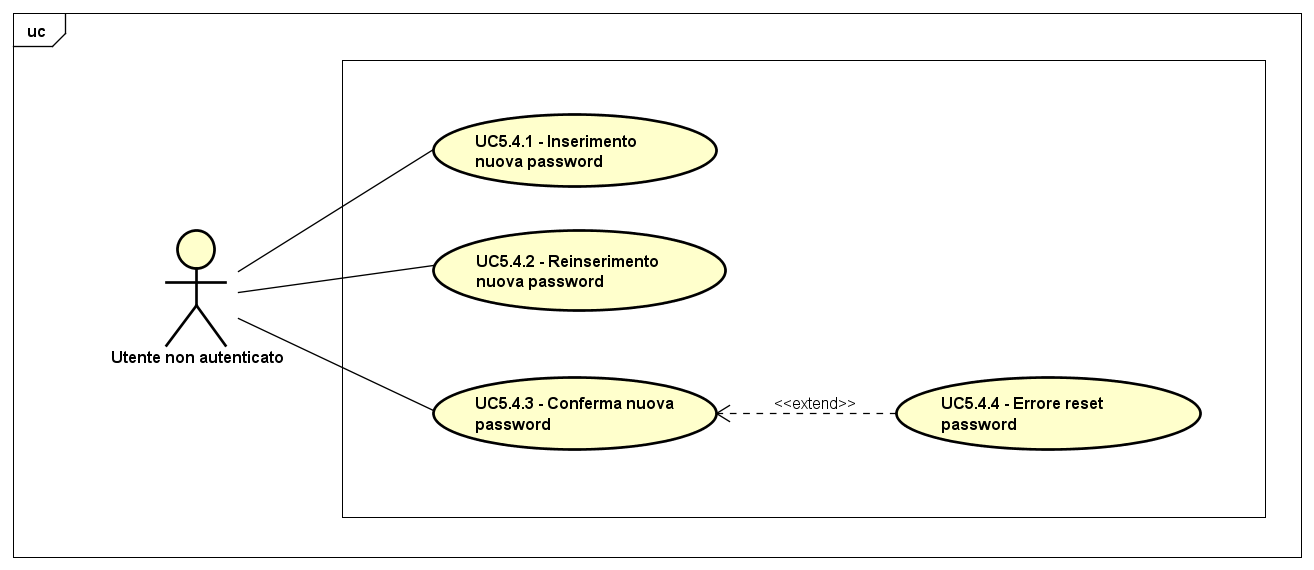
\includegraphics[scale=0.45]{UML/UC5_4.png}
	\caption{UC5.4: Reset password}
\end{figure}

\begin{minipage}{\linewidth}
	\begin{longtable}{ l | p{11cm}}
		\hline
		\rowcolor{Gray}
		\multicolumn{2}{c}{UC5.4 - Reset password} \\
		\hline
		\textbf{Attori} & Utente non autenticato \\
		\textbf{Descrizione} & L'attore ha ricevuto un link per la schermata di reset della propria password \\
		\textbf{Pre-Condizioni} & L'attore ha richiesto il recupero della password ed ha aperto il link per poterla resettare \\
		\textbf{Post-Condizioni} & L'attore ha resettato con successo la password \\
		\textbf{Scenario Principale} & 
		\begin{enumerate*}[label=(\arabic*.),itemjoin={\newline}]
			\item L'attore può inserire la nuova password desiderata (UC5.4.1)
			\item L'attore può reinserire la nuova password desiderata (UC5.4.2)
			\item L'attore può confermare i dati inseriti e completare la procedura con successo (UC5.4.3)
		\end{enumerate*}\\
		\textbf{Scenari Alternativi} & 
		\begin{enumerate*}[label=(\arabic*.),itemjoin={\newline}]
			\item L'attore visualizza un errore qualora le password inserite non coincidano o i campi risultino vuoti (UC5.4.4)
		\end{enumerate*}\\
	\end{longtable}
\end{minipage}

\paragraph{Caso d'uso UC5.4.1: Inserimento nuova password}
\label{UC5_4_1}

\begin{minipage}{\linewidth}
	\begin{longtable}{ l | p{11cm}}
		\hline
		\rowcolor{Gray}
		\multicolumn{2}{c}{UC5.4.1 - Inserimento nuova password} \\
		\hline
		\textbf{Attori} & Utente non autenticato \\
		\textbf{Descrizione} & L'attore inserisce la nuova password per il proprio account \\
		\textbf{Pre-Condizioni} & L'applicazione mostra la schermata di reset password \\
		\textbf{Post-Condizioni} & L'attore ha inserito la nuova password \\
		\textbf{Scenario Principale} & 
		\begin{enumerate*}[label=(\arabic*.),itemjoin={\newline}]
			\item L'attore può inserire la nuova password per il proprio account
		\end{enumerate*}\\
	\end{longtable}
\end{minipage}

\paragraph{Caso d'uso UC5.4.2: Reinserimento nuova password}
\label{UC5_4_2}

\begin{minipage}{\linewidth}
	\begin{longtable}{ l | p{11cm}}
		\hline
		\rowcolor{Gray}
		\multicolumn{2}{c}{UC5.4.2 - Reinserimento nuova password} \\
		\hline
		\textbf{Attori} & Utente non autenticato \\
		\textbf{Descrizione} & L'attore reinserisce la nuova password per il proprio account \\
		\textbf{Pre-Condizioni} & L'applicazione mostra la schermata di reset password \\
		\textbf{Post-Condizioni} & L'attore ha reinserito la nuova password \\
		\textbf{Scenario Principale} & 
		\begin{enumerate*}[label=(\arabic*.),itemjoin={\newline}]
			\item L'attore può reinserire la nuova password per il proprio account
		\end{enumerate*}\\
	\end{longtable}
\end{minipage}

\paragraph{Caso d'uso UC5.4.3: Conferma nuova password}
\label{UC5_4_3}

\begin{minipage}{\linewidth}
	\begin{longtable}{ l | p{11cm}}
		\hline
		\rowcolor{Gray}
		\multicolumn{2}{c}{UC5.4.3 - Conferma nuova password} \\
		\hline
		\textbf{Attori} & Utente non autenticato \\
		\textbf{Descrizione} & L'attore conferma i dati inseriti per poter resettare la propria password \\
		\textbf{Pre-Condizioni} & L'applicazione mostra la schermata di reset password \\
		\textbf{Post-Condizioni} & L'attore ha confermato i nuovi dati per il proprio account \\
		\textbf{Scenario Principale} & 
		\begin{enumerate*}[label=(\arabic*.),itemjoin={\newline}]
			\item L'attore può confermare i nuovi dati per il proprio account, visualizzando un messaggio di successo e venendo reindirizzato alla schermata principale (UC1)
		\end{enumerate*}\\
	\end{longtable}
\end{minipage}

\paragraph{Caso d'uso UC5.4.4: Errore reset password}
\label{UC5_4_4}

\begin{minipage}{\linewidth}
	\begin{longtable}{ l | p{11cm}}
		\hline
		\rowcolor{Gray}
		\multicolumn{2}{c}{UC5.4.4 - Errore reset password} \\
		\hline
		\textbf{Attori} & Utente non autenticato \\
		\textbf{Descrizione} & L'attore conferma i dati inseriti per poter resettare la propria password \\
		\textbf{Pre-Condizioni} & L'attore ha confermato i dati inseriti per poter resettare la propria password \\
		\textbf{Post-Condizioni} & L'attore non ha confermato con successo i propri nuovi dati di accesso \\
		\textbf{Scenario Principale} & 
		\begin{enumerate*}[label=(\arabic*.),itemjoin={\newline}]
			\item L'attore visualizza un messaggio di errore poiché le password non coincidono o i campi sono vuoti
		\end{enumerate*}\\
	\end{longtable}
\end{minipage}